%
% chapter.tex -- Kapitel über endliche Körper
%
% (c) 2021 Prof Dr Andreas Müller, OST Ostschweizer Fachhochschule
%
\chapter{Endliche Körper
\label{buch:chapter:endliche-koerper}}
\lhead{Endliche Körper}
\rhead{}
Aus den ganzen Zahlen $\mathbb{Z}$ entsteht ein Körper, indem wir Brüche
bilden alle von $0$ verschiedenen Nenner zulassen.
Der Körper der rationalen Zahlen $\mathbb{Q}$ enthält unendliche
viele Zahlen und hat zusätzlich die sogenannte archimedische Eigenschaft,
nämliche dass es zu zwei positiven rationalen Zahlen $a$ und $b$ immer eine
ganze Zahl $n$ gibt derart, dass $na>b$.
Dies bedeutet auch, dass es in den rationalen Zahlen beliebig grosse Zahlen
gibt.
Man kann aus den ganzen Zahlen aber auch eine Reihe von Körpern ableiten,
die diese Eigenschaft nicht haben.
Nicht überraschend werden die ersten derartigen Körper, die wir
in Abschnitt~\ref{buch:section:galoiskoerper} konstruieren werden,
endlich viele Elemente haben.
Zu diesen sogenannten Galois-Körpern können wir dann weitere Elemente
hinzufügen, wie das in Abschnitt ~\ref{buch:section:wurzeln} 
gezeigt wird.
Diese Technik, die auch für den Körper $\mathbb{Q}$ funktioniert, erlaubt
dafür zu sorgen, dass in einem Körper gewisse algebraische Gleichungen
lösbar werden.


%
% galois.tex -- Abschnitt über Galois-Körper
%
% (c) 2020 Prof Dr Andreas Müller, Hochschule Rapperswil
%
\section{Galois-Körper
\label{buch:section:galoiskoerper}}
\rhead{Galois-Körper}
Ein Körper $\Bbbk$ enthält mindestens die Zahlen $0$ und $1$.
Die Null ist nötig, damit $\Bbbk$ eine Gruppe bezüglich der
Addition ist, die immer ein neutrales Element, geschrieben $0$
enthält.
Die Eins ist nötig, damit $\Bbbk^*=\Bbbk\setminus\{0\}$ eine
Gruppe bezüglich der Multiplikation ist, die immer eine neutrales
Element, geschrieben $1$ enthält.
Durch wiederholte Addition entstehen auch die Zahlen $2=1+1$, $3=2+1$ 
und so weiter.
Es sieht also so aus, als ob ein Körper immer unendliche viele
Elemente enthalten müsste.
Wie können also endliche Körper entstehen?

In diesem Abschnitt sollen die sogenannten Galois-Körper $\mathbb{F}_p$
mit genau $p$ Elementen konstruiert werden, die es für jede Primzahl $p$ gibt.
Sie sind die Basis für weitere endliche Körper, die eine beliebige
Primzahlpotenz $p^n$ von Elementen haben und die die Basis wichtiger
kryptographischer Algorithmen sind.

%
% Arithmetik module $o$
%
\subsection{Arithmetik modulo $p$
\label{buch:subsection:arithmetik-modulo-p}}
Damit aus den Zahlen $0, 1, 2, \dots$ ein endlicher Körper werden kann,
muss die Folge sich wiederholen.
Schreiben wir $a_0=0,a_1=1,\dots$ für die Folge, dann muss es also
ein Folgenelement $a_k$ geben und ein $n$ derart, dass $a_{k+n}=a_{k}$.
Dies bedeutet, dass $k+n = k$ sein muss.
Subtrahiert man $k$ auf beiden Seiten, dann folgt, dass $n=0$ sein muss.
Damit ein endlicher Körper entsteht, muss also die Menge
\begin{align*}
&\{0,1,2,\dots,n-1\}
\intertext{eine Gruppe bezüglich der Addition sein, und}
&\{1,2,\dots,n-1\}
\end{align*}
eine Gruppe bezüglich der Multiplikation.

\subsubsection{Restklassenring}
Wir definieren die Grundoperationen in einer Menge, die mit den
Zahlen $\{0,1,2,\dots,n-1\}$ identifiziert werden kann.

\begin{definition}
Die Zahlen $a,b\in\mathbb{Z}$ heissen {\em kongruent modulo $n$},
geschrieben
\[
a\equiv b\mod n,
\]
wenn $a-b$ durch $n$ teilbar ist, also $n|(a-b)$.
\end{definition}

Die Zahlen mit gleichem Rest sind Äquivalenzklassen der Kongruenz modulo $n$.
Die Zahlen mit Rest $k$ modulo $n$ bilden die {\em Restklasse}
\[
\llbracket k\rrbracket=\{\dots,k-2n,k-n,k,k+n,k+2n,\dots\} \subset\mathbb{Z}.
\]
Sie bilden eine endliche Menge, die man mit den Resten $0,1,\dots,n-1$
identifizieren kann.

\begin{definition}
Die Menge $\mathbb{Z}/n\mathbb{Z}$ besteht aus den Restklassen
$\llbracket 0\rrbracket,\llbracket 1\rrbracket,\dots,\llbracket n-1\rrbracket$,
die auch einfach $0,1,\dots,n-1$ geschrieben werden.
\end{definition}

Beim Rechnen mit Resten modulo $n$ können Vielfache von $n$ ignoriert werden.
Zum Beispiel gilt 
\[
\begin{aligned}
48&\equiv -1\mod 7& 48&=-1&&\text{in $\mathbb{Z}/7\mathbb{Z}$}
\\
3\cdot 5=15&\equiv 1\mod 7 & 3\cdot 5&=1&&\text{in $\mathbb{Z}/7\mathbb{Z}$.}
\end{aligned}
\]
Das Beispiel zeigt, dass man mindestens in $\mathbb{Z}/7\mathbb{Z}$ mit
Resten ganz ähnlich rechnen kann wie in $\mathbb{Q}$.
In $\mathbb{Z}/7\mathbb{Z}$ scheinen $3$ und $5$ multiplikative inverse
zu sein.

Tatsächlich kann man auf den Restklassen eine Ringstruktur definieren.
Dazu muss man sicherstellen, dass die Auswahl eines Repräsentanten keinen
Einfluss auf den Rest hat.
Der Rest $a$ kann jede Zahl der Form $a+kn$ darstellen.
Ebenso kann der Rest $b$ jede zahl der Form $b+ln$ darstellen.
Deren Summe ist $a+b+(k+l)n\equiv a+b\mod n$.
Der Repräsentant des Restes hat also keinen Einfluss auf die Summe.

Ebenso ist das Produkt der beiden Repräsentaten 
$(a+kn)\cdot(b+ln) = ab + (al+bk)n + kln^2=ab + (al+bk+kln)n\equiv ab\mod n$
für jede Wahl von $k$ und $l$.
Auch die Multiplikation ist also unabhängig vom gewählten Repräsentanten.

\begin{definition}
Die Menge $\mathbb{Z}/n\mathbb{Z}$ ist ein Ring,
heisst der {\em Restklassenring modulo $n$}.
\end{definition}

\subsubsection{Division in $\mathbb{Z}/n\mathbb{Z}$}
Um einen endlichen Körper zu erhalten, muss die Menge
\[
\mathbb{Z}/n\mathbb{Z} \setminus \{\llbracket0\rrbracket\}
=
\{
\llbracket 1\rrbracket,
\llbracket 2\rrbracket,
\dots
\llbracket n-q\rrbracket
\}
\]
eine Gruppe bezüglich der Multiplikation sein.
Insbesondere darf kein Produkt $a\cdot b$ mit Faktoren in 
$\mathbb{Z}/n\mathbb{Z} \setminus \{\llbracket0\rrbracket\}$
zu Null werden.
Für $n=15$ funktioniert dies nicht, das Produkt $3\cdot 5\equiv 0\mod 15$.
Man nennt von Null verschiedene Faktoren, deren Produkt Null ist, einen
{\em Nullteiler}.
Falls sich $n=p_1\cdot p_2$ in zwei Faktoren zerlegen lässt, dann sind
$p_1$ und $p_2$ Nullteiler in $\mathbb{Z}/n\mathbb{Z}$.
Ein Körper kann also nur entstehen, wenn $n$ eine Primzahl ist.

\begin{definition}
Ist $p$ eine Primzahl, dann heisst $\mathbb{F}_p=\mathbb{Z}/p\mathbb{Z}$
der Galois-Körper der Ordnung $p$.
\end{definition}

Diese Definition ist nur gerechtfertigt, wenn $\mathbb{F}_p^*$ tatsächlich
eine Gruppe ist, wenn also jede Zahl zwischen $1$ und $p-1$ ein Inverses
bezüglich der Multiplikation hat.
Zu einem Rest $a\in\mathbb{F}_p^*$ muss also ein Rest $b$ gefunden werden,
so dass $ab\equiv 1\mod p$.
Dies ist gleichbedeutend mit Zahlen $b$ und $n$ derart, dass
\begin{equation}
ab+np=1.
\label{buch:endliche-koerper:teilerfremd}
\end{equation}
In~\eqref{buch:endliche-koerper:teilerfremd} sind $a$ und $p$ gegeben,
gesucht sind $b$ und $n$.

In Abschnitt~\ref{buch:section:euklid} wurde gezeigt, wie der euklidische
Algorithmus eine Gleichung der Form~\eqref{buch:endliche-koerper:teilerfremd}
lösen kann, wenn die beiden gegebenen Zahlen $a$ und $p$ teilerfremd sind.
Dies ist aber dadurch garantiert, dass $p$ eine Primzahl ist und $1\le a <p$.
Die multiplikative Inverse von $a$ in $\mathbb{F}_p^*$ kann also mit
Hilfe des euklidischen Algorithmus effizient gefunden werden.

\begin{beispiel}
Die kleinste Primzahl grösser als $2021$ ist $p=2063$.
Was ist die Inverse von $2021$ in $\mathbb{F}_{2063}$?

Wir führen den euklidischen Algorithmus für das Paar $(2063,2021)$ durch
und erhalten 
\begin{center}
\begin{tabular}{|>{$}c<{$}|>{$}r<{$}|>{$}r<{$}|>{$}r<{$}|>{$}r<{$}|}
\hline
k&  a_k&  b_k& q_k& r_k\\
\hline
0& 2063& 2021&   1&  42\\
1& 2021&   42&  48&   5\\
2&   42&    5&   8&   2\\
3&    5&    2&   2&   1\\
4&    2&    1&   2&   0\\
\hline
\end{tabular}
\end{center}
Die gesuchten Faktoren $b$ und $n$ können aus dem Matrizenprodukt
$Q(q_n)\dots Q(q_0)$ gefunden werden:
\begin{align*}
Q
&=
\begin{pmatrix} 0& 1\\ 1& -2 \end{pmatrix}
\begin{pmatrix} 0& 1\\ 1& -2 \end{pmatrix}
\begin{pmatrix} 0& 1\\ 1& -8 \end{pmatrix}
\begin{pmatrix} 0& 1\\ 1& -48 \end{pmatrix}
\begin{pmatrix} 0& 1\\ 1& -1 \end{pmatrix}
\\
&=
\begin{pmatrix} 0& 1\\ 1& -2 \end{pmatrix}
\begin{pmatrix} 0& 1\\ 1& -2 \end{pmatrix}
\begin{pmatrix} 0& 1\\ 1& -8 \end{pmatrix}
\begin{pmatrix} 1& -1\\ -48& 49\end{pmatrix}
\\
&=
\begin{pmatrix} 0& 1\\ 1& -2 \end{pmatrix}
\begin{pmatrix} 0& 1\\ 1& -2 \end{pmatrix}
\begin{pmatrix} -48& 49\\ 385& -393 \end{pmatrix}
\\
&=
\begin{pmatrix} 0& 1\\ 1& -2 \end{pmatrix}
\begin{pmatrix} 385& -393\\ -818& 835 \end{pmatrix}
\\
&=
\begin{pmatrix} -818&   835\\ 2021& -2063\end{pmatrix}
\end{align*}
Daraus können wir ablesen, dass
\[
-818\cdot 2021 +835 \cdot 2063=1.
\]
Der Rest $ -818\equiv 1245\mod 2063$ ist also die multiplikative
Inverse von $2021$ in $\mathbb{F}_{2063}$.
\end{beispiel}

\subsubsection{Der kleine Satz von Fermat}
In $\mathbb{Z}$ wachsen die Potenzen einer Zahl immer weiter an.
In einem endlichen Körper kann dies nicht gelten, da nur endlich
viele Werte zur Verfügung stehen.
Tatsächlich müssen die Potenzen einer von $0$ verschiedenen Zahl
$a\in\mathbb{F}_p^*$ alle in $\mathbb{F}_p^*$ liegen.
Es gibt aber nur $p-1$ Zahlen in $\mathbb{F}_p^*$, spätestens
die Potenz mit Exponent $p$ muss also mit einer früheren Potenz
übereinstimmen.
Der kleine Satz von Fermat sagt etwas genauer: die $p$-te Potenz
von $a$ ist genau die Zahl $a$:

\begin{satz}[Kleiner Satz von Fermat]
\label{buch:endliche-koerper:satz:fermat}
In $\mathbb{F}_p$ gilt $a^p=a$ für alle $a\in\mathbb{F}_p^*$.
\end{satz}

Wir beweisen diesen Satz in der folgenden, traditionelleren 
Formulierung.

\begin{satz}
Für jede ganze Zahl $a>0$ gilt $p|(a^p-a)$ genau dann, wenn
$p$ eine Primzahl ist.
\end{satz}

\begin{proof}[Beweis]
Wir müssen zeigen, dass $p$ ein Teiler ist von $a^p-a$.
Das nachfolgende kombinatorische Argument wird zum Beispiel
von Mathologor auf seinem Youtube-Kanal im Video
\url{https://youtu.be/_9fbBSxhkuA} illustriert.

Zum Beiweis interpretieren wir die vorkommenden Zahlen kombinatorisch.
Die Zahl $a^p$ ist die Anzahl der verschiedenen Perlenketten der Länge
$p$, die sich aus Glasperlen mit $a$ verschiedenen Farben herstellen
lassen.
Davon bestehen $a$ Perlenketten aus nur einer einzigen Farbe.
Die Zahl $a^p-a$ ist also die Anzahl der Perlenketten der Länge $p$
aus Glasperlen mit $a$ verschiedenen Farben, die mindestens zwei
verschiedene Farben verwenden.

Wir stellen jetzt die Frage nach der Anzahl der geschlossenen
Perlenketten der Länge $p$ als Glasperlen in $a$ verschiedenen Farben.
Aus jeder geschlossenen Perlenkette lassen sich $p$ Perlenketten machen,
indem man sie an einer der $p$ Trennstellen zwischen Perlen aufteilt.

Wir müssen uns noch überlegen, unter welchen Voraussetzungen 
alle diese möglichen Auftrennungen zu verschiedenen Perlenketten
führen.
Zwei Trennstellen, die $k$-Perlen auseinander liegen, führen nur dann
zur gleichen Perlenkette, wenn die geschlossenen Ketten durch Drehung 
um $k$ Perlen ineinander umgehen.
Dies bedeutet aber auch, dass sich das Farbmuster alle $k$-Perlen
wiederholen muss.
Folglich ist $k$ ein Teiler von $p$.
$p$ Verschiedene Perlenketten entstehen also immer genau dann, wenn $p$
eine Primzahl ist.

Wir schliessen daraus, dass $a^p-a$ durch $p$ teilbar ist, genau dann,
wenn $p$ eine Primzahl ist.
\end{proof}

Der kleine Satz von Fermat kann auch dazu verwendet werden, Potenzen 
in $\mathbb{F}_p$ zu vereinfachen, wie das folgende Beispiel\footnote{%
Das Beispiel stammt aus dem Video~\url{https://youtu.be/_9fbBSxhkuA},
welches Mathologer zu Halloween 2018 veröffentlich hat}
zeigt.

\begin{beispiel}
Man berechnet in $\mathbb{F}_{13}$ die Potenz $11^{666}$.
Nach dem kleinen Satz von Fermat ist $11^{13} = 11$ oder $11^{12}=1$,
man kann also den Exponenten modulo $12$ reduzieren.
Weil $666=55\cdot 12 + 6$ erhält man $11^{666}= 11^6$.
Da die Potenzen von $11$ etwas mühsam zu berechnen sind,
kann man sie wegen $11=-2$ in $\mathbb{F}_{13}$ auch als Potenzen
von $-2$ bekommen.
Aber $(-2)^6 = 64 = -1 \in\mathbb{F}_{13}$.
\end{beispiel}

In der Form $a^{p-1}=1$ in $\mathbb{F}_p$ liefert der kleine Satz
von Fermat die Inverse von $a$ als $a^{p-2}$.
Dies bedeutet zum Beispiel, dass in $\mathbb{F}_3$ jede von $0$
verschiedene Zahl zu sich selbst invers ist: $1\cdot 1=1$ und $2\cdot 2=1$.
Diese Art, die Inverse zu bestimmen, ist allerdings nicht effizienter
als der euklidische Algorithmus, aber sie ist manchmal für
theoretische Überlegungen nützlich.

\subsubsection{Der Satz von Wilson}
Der Satz von Wilson ermöglicht, die multiplikative Inverse auf eine
andere Art zu berechnen.
Sie ist zwar nicht unbedingt einfacher, aber manchmal nützlich für
theoretische Überlegungen.

\begin{satz}[Wilson]
Die ganze Zahl $p\ge 2$ ist genau dann eine Primzahl, wenn
$(p-1)!\equiv -1\mod p$.
\end{satz}

\begin{proof}[Beweis]
Wenn $p$ keine Primzahl ist, dann lässt sich $p$ in Faktoren
$p=n_1\cdot n_2=p$ zerlegen.
Beide Faktoren kommen in der Liste $1,2,\dots,p-1$ vor.
Insbesondere haben $p=n_1n_2$ und $(p-1)!$ mindestens einen
der Faktoren $n_1$ oder $n_2$ gemeinsam, wir können annehmen,
dass $n_1$ dieser Faktor ist.
Es folgt, dass der grösste gemeinsame Teiler von $p$ und $(p-1)!$
grösser als $n_1$ ist, auch $(p-1)!$ ein Vielfaches von $n_1$ in
$\mathbb{F}_p$.
Insbesondere kann $(p-1)!$ nicht $-1\in\mathbb{F}_p$ sein.

Ist andererseits $p$ eine Primzahl, dann sind die Zahlen $1, 2,\dots,p-1$
alle invertierbar in $\mathbb{F}_p$.
Die Zahlen $1$ und $-1\equiv p-1\mod p$ sind zu sich selbst invers,
da $1\cdot 1=1$ und $(-1)\cdot(-1)=1$.
Wenn eine Zahl $a$ zu sich selbst invers ist in $\mathbb{F}_p$,
dann ist $a^2-1=0$ in $\mathbb{F}_p$.
Daher ist auch $(a+1)(a-1)=0$, in $\mathbb{F}_p$ muss daher einer
der Faktoren $0$ sein, also $a=-1$ oder $a=1$ in $\mathbb{F}_p$.

Zu jeder Zahl $a\in\{2,\dots,p-2\}$ liegt die Inverse $a^{-1}$
ebenfalls in diesen Bereich und ist verschieden von $a$: $a^{-1}\ne a$.
Das Produkt der Zahlen
$2\cdot 3 \cdot\ldots\cdot (p-2)$ besteht also aus zueinander inversen
Paaren.
Es folgt
\[
2\cdot 3 \cdot\ldots\cdot (p-2) = 1.
\]
Multipliziert man dies mit $p-1=-1\in\mathbb{F}_p$, folgt
die Behauptung des Satzes.
\end{proof}

Mit dem Satz von Wilson kann man die Inverse einer beliebigen Zahl
$a\in\mathbb{F}_p$ finden.
Dazu verwendet man, dass $a$ einer der Faktoren in $(p-1)!$ ist.
Lässt man diesen Faktor weg, erhält man eine Zahl
\[
b = 1\cdot 2 \cdot \ldots\cdot \hat{a}\cdot\ldots\cdot (p-1),
\]
wobei der Hut bedeutet, dass der Faktor $a$ weggelassen werden soll.
Nach dem Satz von Wilson ist $ab=-1$ in $\mathbb{F}_p$, also ist
$-b$ die multiplikative Inverse  von $a$.

\begin{beispiel}
Die Inverse von $2\in\mathbb{F}_7$ ist
\begin{align*}
a^{-1}
&=
-\underbrace{1\cdot 3\cdot 4}_{}\cdot \underbrace{5\cdot 6}_{}
\\
&=
-5\cdot 2
=
-3
=4
\end{align*}
Tatsächlich ist $2\cdot 4=8\equiv 1\mod 7$.
\end{beispiel}

%
% Charakteristik
%
\subsection{Charakteristik
\label{buch:subsection:charakteristik}}
In diesem Abschnitt zeigen wir, dass jeder Körper $\Bbbk$ eine Erweiterung
entweder von $\mathbb{Q}$ oder eines endlichen Körpers $\mathbb{F}_p$ ist.

\subsubsection{Primkörper}
Sei $\Bbbk$ ein Körper.
Er enthält mindestens die Zahlen $0$ und $1$ und alle Vielfachen davon.
Wenn alle Vielfachen in $\Bbbk$ von $0$ verschieden sind, dann
bilden Sie ein Bild der ganzen Zahlen $\mathbb{Z}\subset\Bbbk$.
Damit müssen dann aber auch alle Brüche in $\Bbbk$ enhalten sein,
es folgt also, dass $\mathbb{Q}\subset\Bbbk$ sein muss.

Wenn andererseits eines der Vielfachen von $1$ in $\Bbbk$ 
verschwindet, dann wissen wir aus
Abschnitt~\ref{buch:subsection:arithmetik-modulo-p}, dass
der Körper $\mathbb{F}_p$ in $\Bbbk$ enthalten sein muss.
Dies ist der kleinste Teilkörper, der in $\Bbbk$ enthalten ist.

\begin{definition}
Der kleinste Teilkörper eines Körpers $\Bbbk$ heisst der 
{\em Primkörper} von $\Bbbk$.
\end{definition}

Der Primkörper erlaubt jetzt, die Charakteristik eines Körpers $\Bbbk$
zu definieren.

\begin{definition}
Die Charakteristik eines Körpers $\Bbbk$ ist $p$, wenn der Primkörper
$\mathbb{F}_p$ ist.
Falls der Primkörper $\mathbb{Q}$ ist, ist die Charakteristik $0$.
\end{definition}

Die Charakteristik hat wichtige Auswirkungen darauf, wie in einem Körper
gerechnet wird.
Endliche Körper enthalten immer einen Körper von Primzahl-Ordnung und
haben damit immer Primcharakteristik.
Ein Körper mit Charakteristik $0$ enthält immer unendliche viele
Elemente.

\subsubsection{Teilbarkeit von Binomialkoeffizienten}
\begin{figure}
\centering
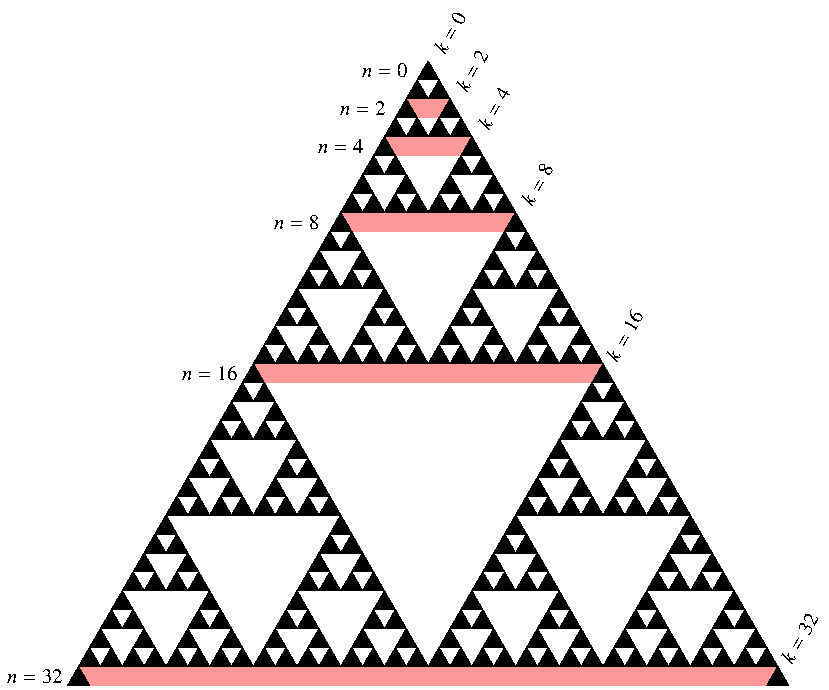
\includegraphics{chapters/30-endlichekoerper/images/binomial2.pdf}
\caption{Binomialkoeffizienten module $2$ im Pascal-Dreieck.
Auf Zeilen, die zu Exponenten der Form $2^k$ gehören, sind alle 
Koeffizienten ausser dem ersten und letzten durch $2$ teilbar.
\label{buch:endliche-koerper:fig:binomial2}}
\end{figure}
Die Abbildung~\ref{buch:endliche-koerper:fig:binomial2} zeigt den
Rest bei Teilung durch $2$ der Binomialkoeffizienten.
Man kann daraus ablesen, dass $\binom{n}{m}\equiv 0\mod 2$ für $n=2^k$ 
und $0<m<n$.

\begin{satz}
\label{buch:endliche-koerper:satz:binom}
Sei $p$ eine Primzahl, dann ist
\[
\binom{p}{m} \equiv 0\mod p
\]
für $0<m<n$.
\end{satz}

\begin{proof}[Beweis]
Für den Binomialkoeffizienten gilt
\[
\binom{p}{m}
=
\frac{p\cdot (p-1)\cdot(p-2)\cdot\ldots\cdot (p-m+1)}{1\cdot 2\cdot 3\cdot\ldots\cdot m}.
\]
Für $m<p$ kann keiner der Faktoren im Nenner $p$ sein, der Faktor $p$
im Zähler kann also nicht weggekürzt werden, so dass der Binomialkoeffizient
durch $p$ teilbar sein muss.
\end{proof}

Die Aussage von Satz~\ref{buch:endliche-koerper:satz:binom} kann man 
auch im Körper $\mathbb{F}_p$ formulieren:

\begin{satz}
\label{buch:endliche-koerper:satz:binomFp}
In $\mathbb{F}_p$ gilt
\[
\binom{p}{k}=0
\]
für $0<k<p$.
\end{satz}

\subsubsection{Frobenius-Automorphismus}
Die Abbildung $x\mapsto x^n$ ist weit davon entfernt, sich mit den
algebraischen Strukturen zu vertragen.
Zum Beispiel kann man nicht erwarten, dass $(a+b)^n = a^n + b^n$,
denn nach der binomischen Formel
\begin{equation}
(a+b)^n
=
\sum_{k=0}^n \binom{n}{k} a^k b^{n-k}
=
a^n + \binom{n}{1}a^{n-1}b + \dots + \binom{n}{n-1}ab^{n-1} + b^n
\label{buch:endliche-koerper:fig:binomischeformel}
\end{equation}
gibt es zwischen den Termen an den Enden des Ausdrucks noch viele
Zwischenterme, die normalerweise nicht verschwinden.

Ganz anders sieht die Situation aus, wenn $n=p$ ist.
Nach Satz~\ref{buch:endliche-koerper:satz:binomFp} verschwinden die
Binomialkoeffizienten der Zwischenterme der Summe
\eqref{buch:endliche-koerper:fig:binomischeformel}
als Elemente von $\mathbb{F}_p$.
Daher gilt

\begin{satz}[Frobenius-Automorphismus]
In einem Körper $\Bbbk$ der Charakteristik $p$ ist die Abbildung
$x\mapsto x^p$ ist ein Automorphismus, der den Primkörper 
$\mathbb{F}_p\subset\Bbbk$ fest lässt.
\end{satz}

\begin{proof}[Beweis]
Wir müssen uns nur noch davon überzeugen, dass $\mathbb{F}_p\subset\Bbbk$
fest bleibt.
Nach dem kleine Satz von Fermat~\ref{buch:endliche-koerper:satz:fermat}
ist $a^p=a$ für alle $a\in\mathbb{F}_p$, der Frobenius-Automorphismus
lässt also alle Elemente von $\mathbb{F}_p$ fest.
\end{proof}

\begin{definition}
Der Automorphismus $x\mapsto x^p$ heisst {\em Frobenius-Automorphismus}.
\end{definition}

%
% wurzeln.tex -- Wurzeln einem endlichen Körper hinzufügen
%
% (c) 2021 Prof Dr Andreas Müller, Hochschule Rapperswil
%
\section{Wurzeln
\label{buch:section:wurzeln}}
\rhead{Wurzeln}
Im Körper $\mathbb{Q}$ kann man zum Beispiel die Wurzel aus $2$ nicht 
ziehen.
Das Problem haben wir in Abschnitt~\ref{buch:section:reelle-zahlen}
dadurch gelöst, dass wir $\mathbb{Q}$ zu den reellen Zahlen
erweitert haben.
Es ist aber auch möglich, nur die Zahl $\sqrt{2}$ hinzuzufügen,
so entsteht der Körper $\mathbb{Q}(\sqrt{2})$.
In diesem Abschnitt zeigen wir, wie man einem Körper beliebige 
Nullstellen $\alpha$ eines Polynoms $f\in\Bbbk[X]$ hinzufügen und
so den Körper $\Bbbk(\alpha)$ konstruieren kann.

\subsection{Irreduzible Polynome
\label{buch:subsection:irreduziblepolynome}}
Die Zahlen, die man dem Körper hinzufügen möchte, müssen Nullstellen
eines Polynoms sein.
Wir gehen daher davon aus, dass $f\in \Bbbk[X]$ ein Polynom mit
Koeffizienten in $\Bbbk$ ist, dessen Nullstelle $\alpha$ hinzugefügt
werden sollen.
Das Ziel ist natürlich, dass diese Erweiterung vollständig beschrieben
werden kann durch das Polynom, ganz ohne Bezug zum Beispiel auf einen
numerischen Wert der Nullstelle, der ohnehin nur in $\mathbb(C)$ sinnvoll
wäre.

Nehmen wir jetzt an, dass sich das Polynom $f$ faktorisieren lässt.
Dann gibt es Polynome $g,h\in\Bbbk[X]$ derart, dass $f=g\cdot h$.
Die Polynome $g$ und $h$ haben geringeren Grad als $f$. 
Setzt man die Nullstelle $\alpha$ ein, erhält man
$0=f(\alpha)=g(\alpha)h(\alpha)$, daher muss einer der Faktoren
verschwinden, also $g(\alpha)=0$ oder $h(\alpha)=0$.
Ohne Beschränkung der Allgemeinheit kann angenommen werden, dass
$g(\alpha)=0$.
Die Operation des Hinzufügens der Nullstelle $\alpha$ von $f$
muss also genauso gut mit $g$ ausgeführt werden.
Indem wir diese Überlegung auf $g$ anwenden können wir schliessen,
dass es ein Polynom $m\in\Bbbk[X]$ kleinstmöglichen Grades geben muss,
welches $\alpha$ als Nullstelle hat.
Zusätzlich kann verlangt werden, dass das Polynom normiert ist.

\begin{definition}
Ein Polynom $f\in \Bbbk[X]$ heisst {\em irreduzibel}, wenn es sich nicht
in zwei Faktoren $g,h\in \Bbbk[X]$ mit $f=gh$ zerlegen lässt.
\index{irreduzibles Polynom}%
\end{definition}

Für die Konstruktion des Körpers $\Bbbk(\alpha)$ muss daher ein irreduzibles
Polynom verwendet werden.

\begin{beispiel}
Das Polynom $f(X)=X^2-2$ ist in $\mathbb{Q}[X]$, es hat die beiden
Nullstellen $\sqrt{2}$ und $-\sqrt{2}$.
Beide Nullstellen haben die exakt gleichen algebraischen Eigenschaften,
sie sind mit algebraischen Mitteln nicht zu unterscheiden.
Nur die Vergleichsrelation ermöglicht, die negative Wurzel von der
positiven zu unterscheiden.
Das Polynom kann in $\mathbb{Q}$ nicht faktorisiert werden, denn die
einzig denkbare Faktorisierung ist $(X-\sqrt{2})(X+\sqrt{2})$, die
Faktoren sind aber keine Polynome in $\mathbb{Q}[X]$.
Also ist ein irreduzibles Polynom über $X^2-2$.

Man kann das Polynom aber auch als Polynom in $\mathbb{F}_{23}[X]$
betrachten.
Im Körper $\mathbb{F}_{23}$ kann man durch probieren zwei Nullstellen
finden:
\begin{align*}
5^2 &= 25\equiv 2\mod 23
\\
\text{und}\quad
18^2 &=324 \equiv 2 \mod 23.
\end{align*}
Und tatsächlich ist in $\mathbb{F}_{23}[X]$
\[
(X-5)(X-18) = X^2 -23X+90
\equiv
X^2 -2 \mod 23,
\]
über $\mathbb{F}_{23}$ ist das Polynom $X^2-2$ also reduzibel.
\end{beispiel}

\begin{beispiel}
Die Zahl 
\[
\alpha = \frac{1+i\sqrt{3}}2
\]
ist eine Nullstelle des Polynoms $f(X)=X^3-1\in\mathbb{Z}[X]$.
$\alpha$ enthält aber nur Quadratwurzeln, man würde also eigentlich
erwarten, dass $\alpha$ Nullstelle eines quadratischen Polynoms ist.
Tatsächlich ist $f(X)$ nicht irreduzibel,  es ist nämlich
\[
X^3-1 = (X-1)(X^2+X+1).
\]
Da $\alpha$ nicht Nullstelle des ersten Faktors ist, muss es Nullstelle
des Polynoms $m(X)=X^2+X+1$ sein.
Der zweite Faktor ist irreduzibel.

Das Polynom $m(X)$ kann man aber auch als Polynom in $\mathbb{F}_7$ 
ansehen.
Dann kann man aber zwei Nullstellen finden,
\[
\begin{aligned}
X&=2&&\Rightarrow& 2^2+2+1=4+2+1&\equiv 0\mod 7
\\
X&=4&&\Rightarrow& 4^2+4+1=16+4+1=21&\equiv 0\mod 7.
\end{aligned}
\]
Dies führt auf die Faktorisierung
\[
(X-2)(X-4)
\equiv
(X+5)(X+3)
=
X^2+8X+15
\equiv
X^2+X+1\mod 7.
\]
Das Polynom $X^2+X+1$ ist daher über $\mathbb{F}_7$ reduzibel und
das Polynom $X^3-1\in\mathbb{F}_7$ zerfällt daher in Linearfaktoren
$X^3-1=(X+6)(X+3)(X+5)$.
\end{beispiel}


\subsection{Körpererweiterungen}
Nach den Vorbereitungen von
Abschnitt~\ref{buch:subsection:irreduziblepolynome}
können wir jetzt definieren, wie die Körpererweiterung
konstruiert werden soll.

\subsubsection{Erweiterung mit einem irreduziblen Polynom}
Sei $m\in\Bbbk[X]$ ein irreduzibles Polynome über $\Bbbk$ mit dem Grad
$\deg m=n$,
wir dürfen es als normiert annehmen und schreiben es in der Form
\[
m(X)
=
m_0+m_1X+m_2X^2 + \dots m_{n-1}X^{n-1}+X^n.
\]
Wir möchten den Körper $\Bbbk$ um eine Nullstelle $\alpha$ von $m$
erweitern.
Da es in $\Bbbk$ keine Nullstelle von $m$ gibt, konstruieren wir
$\Bbbk(\alpha)$ auf abstrakte Weise, ganz so wie das mit der imaginären
Einheit $i$ gemacht wurde.
Die Zahl $\alpha$ ist damit einfach ein neues Symbol, mit dem man
wie in der Algebra üblich rechnen kann.
Die einzige zusätzliche Eigenschaft, die von $\alpha$ verlangt wird,
ist dass $m(\alpha)=0$.
Unter diesen Bedingungen können beliebige Ausdrücke der Form
\begin{equation}
a_0 + a_1\alpha + a_2\alpha^2 + \dots a_k\alpha^k
\label{buch:endlichekoerper:eqn:ausdruecke}
\end{equation}
gebildet werden.
Aus der Bedingung $m(\alpha)=0$ folgt aber, dass
\begin{equation}
\alpha^n = -a_{n-1}\alpha^{n-1} -\dots - a_2\alpha^2  - a_1\alpha-a_0.
\label{buch:endlichekoerper:eqn:reduktion}
\end{equation}
Alle Potenzen mit Exponenten $\ge n$ in
\eqref{buch:endlichekoerper:eqn:ausdruecke}
können daher durch die rechte Seite von
\eqref{buch:endlichekoerper:eqn:reduktion}
ersetzt werden.
Als Menge ist daher
\[
\Bbbk(\alpha)
=
\{
a_0+a_1\alpha+a_2\alpha^2+\dots+a_{n-1}\alpha^{n-1}\;|\; a_i\in\Bbbk\}.
\}
\]
Die Addition von solchen Ausdrücken und die Multiplikation mit Skalaren
aus $\Bbbk$ machen $\Bbbk(\alpha)\simeq \Bbbk^n$ zu einem Vektorraum,
die Operationen können auf den Koeffizienten komponentenweise ausgeführt
werden.

\subsubsection{Matrixrealisierung der Multiplikation mit $\alpha$}
Die schwierige Operation ist die Multiplikation mit $\alpha$.
Dazu stellen wir zusammen, wie die Multiplikation mit $\alpha$ auf den
Basisvektoren von $\Bbbk(\alpha)$ wirkt:
\[
\alpha\cdot\colon
\Bbbk^n\to\Bbbk
:
\left\{
\begin{aligned}
     1  &\mapsto \alpha   \\
\alpha  &\mapsto \alpha^2 \\
\alpha^2&\mapsto \alpha^3 \\
        &\phantom{m}\vdots\\
\alpha^{n-2}&\mapsto \alpha^{n-1}\\
\alpha^{n-1}&\mapsto \alpha^n = -m_0-m_1\alpha-m_2\alpha^2-\dots-m_{n-1}\alpha^{n-1}
\end{aligned}
\right.
\]
Diese lineare Abbildung hat die Matrix
\[
M_{\alpha}
=
\begin{pmatrix}
0   &    &    &      &   &-m_0    \\
1   & 0  &    &      &   &-m_1    \\
    & 1  & 0  &      &   &-m_2    \\
    &    & 1  &\ddots&   &-m_3    \\
    &    &    &\ddots& 0 &\vdots  \\
    &    &    &      & 1 &-m_{n-2}\\
    &    &    &      &   &-m_{n-1}
\end{pmatrix}
\]
Aufgrund der Konstruktion die Lineare Abbildung $m(M_\alpha)$,
die man erhält, wenn
man die Matrix $M_\alpha$ in das Polynom $m$ einsetzt, jeden Vektor
in $\Bbbk(\alpha)$ zu Null machen.
Als Matrix muss daher $m(M_\alpha)=0$ sein.
Dies kann man auch mit einem Computeralgebra-System nachprüfen.

\begin{beispiel}
In einem früheren Beispiel haben wir gesehen, dass
$\alpha=\frac12(-1+\sqrt{3})$ 
eine Nullstelle des irreduziblen Polynomes $m(X)=X^2+X+1$ ist.
Die zugehörige Matrix $M_\alpha$ ist
\[
M_{\alpha}
=
\begin{pmatrix}
0&-1\\
1&-1
\end{pmatrix}
\qquad\Rightarrow\qquad
M_{\alpha}^2
=
\begin{pmatrix}
-1& 1\\
-1& 0
\end{pmatrix},\quad
M_{\alpha}^3
=
\begin{pmatrix}
 1& 0\\
 0& 1
\end{pmatrix}.
\]
Wir können auch verifizieren, dass
\[
m(M_\alpha)
=
M_\alpha^2+M_\alpha+I
=
\begin{pmatrix}
-1& 1\\
-1& 0
\end{pmatrix}
+
\begin{pmatrix}
0&-1\\
1&-1
\end{pmatrix}
+
\begin{pmatrix}
1&0\\
0&1
\end{pmatrix}
=
\begin{pmatrix}
0&0\\
0&0
\end{pmatrix}.
\]
Die Matrix ist also eine mögliche Realisierung für das ``mysteriöse''
Element $\alpha$.
Es hat alle algebraischen Eigenschaften von $\alpha$.
\end{beispiel}

Die Menge $\Bbbk(\alpha)$ kann durch die Abbildung $\alpha\mapsto M_\alpha$
mit der Menge aller Matrizen
\[
\Bbbk(M_\alpha)
=
\left\{
\left.
a_0I+a_1M_\alpha+a_2M_\alpha^2+\dots+a_{n-1}M_\alpha^{n-1}\;\right|\; a_i\in\Bbbk
\right\}
\]
in eine Eins-zu-eins-Beziehung gebracht werden.
Diese Abbildung ist ein Algebrahomomorphismus.
Die Menge $\Bbbk(M_\alpha)$ ist also das Bild des
Körpers $\Bbbk(\alpha)$ in der Matrizenalgebra $M_n(\Bbbk)$.

\subsubsection{Inverse}
Im Moment wissen wir noch nicht, wie wir $\alpha^{-1}$ berechnen sollten.
Wir können aber auch die Matrizendarstellung verwenden können.
Für Matrizen wissen wir selbstverständlich, wie Matrizen invertiert
werden können.
Tatsächlich kann man die Matrix $M_\alpha$ direkt invertieren:
\[
M_\alpha^{-1}
=
\frac{1}{m_0}
\begin{pmatrix}
   -m_1 &m_0&   &      &      &   \\
   -m_2 & 0 &m_0&      &      &   \\
   -m_3 &   & 0 &   m_0&      &   \\
 \vdots &   &   &\ddots&\ddots&   \\
-m_{n-1}& 0 & 0 &      &  0   &m_0\\
    -1  & 0 & 0 &      &  0   & 0
\end{pmatrix},
\]
wie man durch Ausmultiplizieren überprüfen kann:
\[
\frac{1}{m_0}
\begin{pmatrix}
   -m_1 &m_0&   &      &      &   \\
   -m_2 & 0 &m_0&      &      &   \\
   -m_3 &   & 0 &   m_0&      &   \\
 \vdots &   &   &\ddots&\ddots&   \\
-m_{n-1}& 0 & 0 &      &  0   &m_0\\
    -1  & 0 & 0 &      &  0   & 0
\end{pmatrix}
\begin{pmatrix}
0   &    &    &      &   &-m_0    \\
1   & 0  &    &      &   &-m_1    \\
    & 1  & 0  &      &   &-m_2    \\
    &    & 1  &\ddots&   &-m_3    \\
    &    &    &\ddots& 0 &\vdots  \\
    &    &    &      & 1 &-m_{n-2}\\
    &    &    &      &   &-m_{n-1}
\end{pmatrix}
=
\begin{pmatrix}
1&0&0&\dots&0&0\\
0&1&0&\dots&0&0\\
0&0&1&\dots&0&0\\
\vdots&\vdots&\vdots&\vdots&\vdots\\
0&0&0&\dots&1&0\\
0&0&0&\dots&0&1
\end{pmatrix}
\]
Die Invertierung in $\Bbbk(M_\alpha)$ ist damit zwar geklärt, aber
es wäre viel einfacher, wenn man die Inverse auch in $\Bbbk(\alpha)$
bestimmen könnte.

Die Potenzen von $M_\alpha^k$ haben in der ersten Spalte genau in
Zeile $k+1$ eine $1$, alle anderen Einträge in der ersten Spalte
sind $0$.
Die erste Spalte eines Elementes
$a(\alpha)=a_0+a_1\alpha+a_2\alpha^2 +a_{n-1}\alpha^{n-1}$
besteht daher genau aus den Elementen $a_i$.
Die Inverse des Elements $a$ kann daher wie folgt gefunden werden.
Zunächst wird die Matrix $a(M_\alpha)$ gebildet und invertiert.
Wir schreiben $B=a(M_\alpha)^{-1}$.
Aus den Einträgen der ersten Spalte kann man jetzt die Koeffizienten
\[
b_0=(B)_{11},
b_1=(B)_{21},
b_2=(B)_{11},\dots,
b_{n-1}=(B)_{n,1}
\]
ablesen und daraus das Element
\[
b(\alpha) = b_0+b_1\alpha+b_2\alpha^2 + \dots + b_{n-1}\alpha^{n-1}
\]
bilden.
Da $b(M_\alpha)=B$ die inverse Matrix von $a(M_\alpha)$ ist, muss $b(\alpha)$
das Inverse von $a(\alpha)$ sein.

\begin{beispiel}
Wir betrachten das Polynom 
\[
m(X) = X^3 + 2X^2 + 2X + 3 \in \mathbb{F}_{7}[X],
\]
es irreduzibel.
Sei $\alpha$ eine Nullstelle von $m$, wir suchen das inverse Element zu
\[
a(\alpha)=1+2\alpha+2\alpha^2\in\mathbb{F}_{7}(\alpha).
\]
Die Matrix $a(M_\alpha)$ bekommt die Form
\[
A=\begin{pmatrix}
 1& 1& 6\\
 2& 4& 5\\
 2& 5& 1
\end{pmatrix}.
\]
Die Inverse kann man bestimmen, indem man den
Gauss-Algorithmus in $\mathbb{F}_{17}$ durchführt.
Man bekommt
\[
B=\begin{pmatrix}
 0& 6& 5\\
 6& 4& 0\\
 5& 3& 5
\end{pmatrix}.
\]
Daraus können wir jetzt das inverse Element
\[
b(\alpha) = 6\alpha+5\alpha^2
\]
ablesen.
Das Produkt $b(X)\cdot a(X)$ ist
\begin{align*}
(1+2X+2X^2)(6X+5X^2)
&=
10X^4 + 22X^3 + 17X^2 + 6X
\\
&=
3X^4+X^3+3X^2+6X
\intertext{
Diese Polynom muss jetzt mit dem Minimalpolynom $m(X)$ reduziert
werden, wir subtrahieren dazu $3Xm(X)$ und erhalten}
&=
-5X^3-3X^2-3X
\\
&=
2X^3+4X^2+4X
\intertext{Die vollständige Reduktion wird erreicht, indem wir nochmals
$2m(X)$ subtrahieren:}
&=
-6 \equiv 1\mod 7,
\end{align*}
das Element $b(\alpha)=6\alpha+5\alpha^2$ ist also das Inverse Element von
$a(\alpha)=1+2\alpha+2\alpha^2$ in $\mathbb{F}_7(\alpha)$.
\end{beispiel}

\subsubsection{Rechnen in $\Bbbk(\alpha)$}

\subsubsection{Algebraische Konstruktion}

\subsection{Zerfällungskörper}








